\documentclass{article}
\usepackage[utf8]{inputenc}
\usepackage{amsmath}
\usepackage{amsfonts}
\usepackage{graphicx}
\usepackage{todonotes}
\usepackage{tikz}
\usepackage{gensymb}
\usepackage{amssymb}
\newcommand{\acc}{\text{acc}}
\newcommand{\conf}{\text{conf}}
\newcommand{\D}{\mathcal{D}}
\DeclareMathOperator*{\argmax}{\text{argmax}}
\DeclareMathOperator*{\E}{\mathbb{E}}
\newcommand{\loss}{\mathcal{L}}
\usepackage{hyperref}
\hypersetup{
    colorlinks=true,
    linkcolor=blue,
    filecolor=magenta,      
    urlcolor=blue,
    pdftitle={Overleaf Example},
    pdfpagemode=FullScreen,
}

\title{Out of Distribution Detection}

\begin{document}

\maketitle

\section{Introduction}
One common project within the machine learning community involves developing an image classifier for distinguishing cats and dogs. Students practice building a convolutional base, gluing a few fully connected layers on top, and training on a \href{https://www.kaggle.com/c/dogs-vs-cats}{Kaggle dataset}. Some ambitious students may even deploy their classifier using a phone app for a real-world pet classifier. Yet upon collision with the real world, their model fails in a very predictable way. When fed an image of a hamster, the classifier is unable to answer “hamster” but must output a probability distribution of the “cat” and “dog” options. Any answer which the classifier produces will therefore be meaningless. 

The image of a hamster is considered “out-of-distribution” (OOD) \todo{How often should I use the acronym?} for a cats-and-dogs classifier. It is an example of a way that the testing distribution differs from the training distribution. This example image is indescribable by the model. However, even if this weren’t the case, OOD examples often reduce the quality of model outputs. Perhaps the classifier is trained only on certain breeds of cats. When testing on an unseen breed, the classifier will find it more difficult to generalize—often achieving lower accuracy than expected.

One approach to dealing with out-of-distribution examples is to do ``out-of-distribution detection'' (OOD detection). We build mechanisms into the model so that the model produces both a prediction and a confidence score. Then we set the threshold to a certain point such that any input which produces a lower confidence score is flagged as an OOD example. In such cases, external systems can audit the prediction of the model, potentially discarding or overriding it. Through OOD detection, we minimize the threat that OOD examples pose. 

\section{Problem}
To be precise, we have some model $f_\theta(x)$ which outputs a result and an auxiliary confidence score for each input. We train this model on some dataset $\D^{train}$ and test it on a testing set $\D^{test}$. Because we have access to the training set, we know that $\D^{train}$ consists of only in-distribution data. However, to simulate real-world conditions, we have that $\D^{test}$ is composed of an in-distribution set $\D_{in}^{test}$ and an out-of-distribution set $\D_{out}^{test}$ shuffled together.

Let $s_1, ..., s_n$ and $s’_1, …, s’_n$ be the confidence scores for $\D_{in}^{test}$ and $\D_{out}^{test}$ respectively. Out of distribution detection involves ensuring that the distribution $s_1, …, s_n$ is maximally far from $s’_1, …, s’_n$. Then all scores above a certain threshold $t$ are considered out-of-distribution, whereas all scores below $t$ are considered in-distribution. In practice, the threshold $t$ is not fixed but dynamically generated based on the score distribution of the training set (e.g., the 95\% percentile of $\D^{test}_{in}$). We begin by establishing a few metrics and then discuss common benchmarks that people use.

\subsection{Metrics}
In OOD detection, there are a few specialized metrics that we use. Noticeably, accuracy is not a common metric. The issue with accuracy is that out-of-distribution examples may be really rare. If only 1\% of the data is out-of-distribution, then a model which predicts ``in-distribution'' for each data point will have a 99\% accuracy. In other words, total accuracy is a bad metric for rare events. Instead, OOD detection traditionally uses other metrics. In these notes we focus on the two most common: FPR 95 and AUROC.

\subsubsection{Prerequisites}
To understand these metrics, we first must understand two concepts: false positive rate and true positive rate. Our context is analogous to running a test on different images to detect out-of-distribution examples. A ``positive'' means an image has been marked as out-of-distribution, whereas a ``negative'' means an image has been marked as in-distribution. False positive rate is the proportion of positives which should be negatives (e.g., the proportion of positives in which the image is actually in-distribution). True positive rate is the probability that an out-of-distribution image will be positive (that the image which should be positive actually gets marked positive).

\subsubsection{FPR 95}
One of the primary metrics to measure OOD detection quality is FPR 95, which shows false positive rate at 95\% true positive rate. Essentially, we set the out-of-distribution threshold $t$ such that we detect 95\% of the out-of-distribution data $\D_{out}^{test}$. Then, out of the examples marked as out-of-distribution, we measure the proportion which are actually in-distribution $\D_{in}^{test}$. 

For instance, in the cats-vs-dogs example, we might collect a dataset of cats and dogs $\D_{in}^{test}$ and a dataset of hamsters $\D_{out}^{test}$. Then for FPR 95, we find the threshold $t$ which classifies 95\% of the hamsters as out-of-distribution. Finally, we see the proportion of cat/dog images which as classified as out-of-distribution along with the hamsters. Note that the 95\% threshold is somewhat arbitrary. Other papers have used FPR 90 and, in principle, any FPR $N$ could exist. However, FPR 95 is the current community standard.

\todo{figure}

\begin{figure}
    \centering
    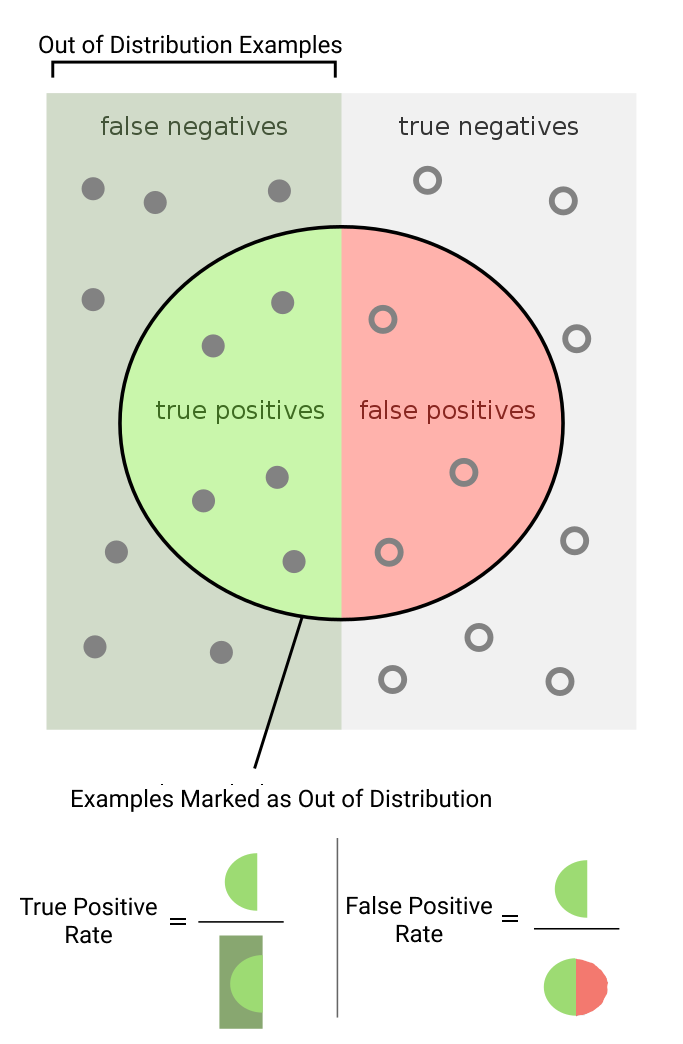
\includegraphics[width=5.5cm]{images/fpr_tpr.png}
    \caption{True positive rate vs false positive rate.}
    \label{fig:my_label}
\end{figure}

\subsubsection{AUROC}
The issue with FPR 95 is that the 95 threshold is somewhat arbitrary and doesn't reflect the model's OOD detection abilities over all other thresholds. Another metric, AUROC, fixes this by being threshold-invariant. Specifically, the receiver operating curve (ROC) is the curve which graphs the true positive rate against the false positive rate. The area under the ROC (AUROC) measures the total area under the curve. Whereas FPR 95 corresponds to one point (one threshold), AUROC incorporates the model's OOD detection over all thresholds. See figure \todo{Fig} for a visualization of this effect. AUROC can also be interpreted as the probability that a clean image has a higher confidence score than an anomaly. An AUROC of 0.5 is random, and an AUROC of 1.0 corresponds to a completely solved task. 

\subsection{Benchmarks}

Unlike other disciplines which require the careful curation of datasets, out-of-distribution detection doesn’t need carefully crafted benchmarks. Simply take two datasets, label one as in-distribution and one as out-of-distribution, and \textit{voila!}, an out-of-distribution detection benchmark is formed. Alternatively, another common way to generate out-of-distribution detection benchmarks is to train a model to recognize only a single class within a dataset. All other examples from all other classes are treated as out-of-distribution. This technique is dubbed \textit{one-class classification} and is unique in that it requires unsupervised out-of-distribution detection methods. (This fact is because all the in-distribution examples the model sees is from the same class.)

This ease of creation means that out-of-distribution detection can be applied to many different domains—images, text, audio, genomic data, etc. However, it also means that setting up common standards of comparison is a bit more difficult than usual. For now, we focus on the canonical set of image classification datasets. Keep in mind that the right benchmarks to evaluate on will differ from domain to domain.

\subsubsection{Image Classification}
In image classification, OOD detection methods are validated on a variety of small datasets (32x32 pixels). Common datasets for this small-scale evaluation include Cifar10 \cite{krizhevsky09learning}, Cifar100 \cite{krizhevsky09learning}, Street View House Numbers (SVHN) \cite{netzer2011reading}, TinyImageNet \cite{le2015tiny}, Large-scale Scene Understanding (LSUN) \cite{yu2016lsun}. Usually, either Cifar10 or SVHN is in-distribution and the remaining are out-of-distribution. Cifar10 is also commonly used for one-class classification. In general, the more similar the two datasets are, the more difficult OOD detection is. For example, when training on Cifar10, detecting SVHN outliers is easier than Cifar100 outliers. At a larger scale, researchers often use ImageNet-1K (the default ImageNet with a thousand classes) \cite{deng2009imagenet}, ImageNet-22K (a superset of ImageNet with 22 thousand classes) \cite{deng2009imagenet}, and LSUN (large scale scene understanding) \cite{yu2016lsun}. Large-scale one-class classification is often done with either ImageNet-1K or ImageNet-22K. Figure \todo{figure} visualizes all of these datasets.

\section{Approaches}

\subsection{Maximum Softmax Probability}
Maximum Softmax Probability (MSP) is an intuitive baseline for finding confidence scores \cite{hendrycks2018baseline}. We simply let the confidence be the maximum of the classifier’s final softmax. For instance, if our cats and dogs classifier outputted a result of [0.8, 0.2], then the MSP confidence would be 0.8. In general, we have that the confidence score $s$ of example $x$ is as follows

\[
     s = \max f_\theta(x)
\]

MSP is a simple method which can sometimes be surprisingly useful. However, usually MSP is ineffective and compared against as a baseline. Outperforming MSP means that, at the very least, your method can outperform the naive solution.

\subsection{Outlier Exposure}
Outlier exposure is a technique to improve out-of-distribution detection algorithms by exposing them to example outliers \cite{hendrycks2019deep}. Consider the example of the cats vs dogs classifier. With outlier exposure, we collect an auxiliary out-of-distribution set, perhaps a dataset of chairs. Then, during training, we teach the model to have low confidence on this auxiliary out-of-distribution set. Finally, during testing, we must test the model’s out-of-distribution detection on out-of-distribution examples that the model has not seen before. Out-of-distribution detection is meant to catch the model’s blind spots which requires testing on new out-of-distribution examples, not ones that the model’s seen before. \todo{figure}

More formally, we now have three datasets, $\D_{in}$, $\D_{out}^{aux}$, $\D_{out}^{test}$. We train the classifier using the in-distribution and the auxiliary dataset using the following loss template:

\[
    \E_{x,y \sim \D_{in}}[\loss(f_\theta(x), y) + \lambda \E_{x' \sim \D_{out}^{aux}} [\loss_{OE}(f_\theta(x'), f_\theta(x), y)]]
\]

\noindent where you can fill $\loss$ and $\loss_{OE}$ in different ways depending on the situation. For image classification, $\loss$ is often cross-entropy and $\loss_{OE}$ often measures the KL divergence between $f_\theta(x')$ and a uniform distribution. 

After training the model, we test out-of-distribution detection on $\D_{out}^{test}$. Interestingly enough, the authors note that $\D_{out}^{aux}$ does not need to be close to $\D_{out}^{test}$ in order for outlier exposure to improve OOD detection. Instead, the auxiliary dataset actually has to be sufficiently close to the in-distribution dataset, $\D_{in}$, so that the classifier doesn’t simply learn very simple patterns. Beyond that, the diversity of the auxiliary dataset also matters. The more diverse the auxiliary dataset, the better the model understands what counts as in-distribution and out-of-distribution.

\subsection{Generative Modeling}

Generative models can also be used for out-of-distribution detection; however, they seem less useful than discriminative methods. There are two ways to use generative models for OOD detection. The first involves generating OOD images and training one’s classifier to have less certainty on these images \cite{lee2018training}. Although moderately effective, simply doing outlier exposure using a diverse auxiliary set outperforms this method.

The second way to use generative models are to leverage the generative model’s likelihood scores directly as a measure of uncertainty. You can use flows \cite{nalisnick2019deep, kirichenko2020normalizing}, autoregressive/feedfoward models \cite{nalisnick2019deep, chen2020generative}, energy-based models \cite{liu2021energybased}, or even variational autoencoders \cite{nalisnick2019deep, xiao2020likelihood}. \footnote{At the time of writing, score based models have not yet been extensively tested.} Each of these can take an image and produce a confidence score. However, one common pattern is that likelihood scores also degrade on out-of-distribution inputs, with generative models sometimes giving higher likelihood to out of distribution images \cite{nalisnick2019deep, choi2019waic, kirichenko2020normalizing}. Currently, this phenomena is not well-understood, although some have argued that it is a consequence of the generative models' inductive biases \cite{kirichenko2020normalizing}. Either way, papers which use generative models are forced to propose tricks to get the out-of-distribution detection working. These tricks provide moderate increases in performance but do not trump the state-of-the-art discriminative out-of-distribution detection methods. 

There are two major exceptions to this pattern. To start, one energy-based method incorporate an outlier exposure approach and explicitly trains on out-of-distribution examples \cite{liu2021energybased}. This approach is shown to outperform outlier exposure. Additionally, [iGPT].

\subsection{Self Supervised Learning}
Another approach to OOD detection involves using self-supervised learning to measure whether the model understands the internal structure within the data \cite{hendrycks2019using, tack2020csi, yoon2021self}. Self-supervised learning involves generating a supervised learning task without any external labels, using only the unlabeled data. For instance, one self-supervised learning task might involve taking a set of images, rotating them $0 \degree, 90 \degree, 180 \degree$, or $270\degree$, and using your model to predict the rotation. Effectively, self-supervised learning measures whether a model understands the internal structure of the data. Then, performance on the self-supervised learning task is a good measure of out-of-distribution. As images become more and more out of distribution, the model understands the internal structure of the image less and less, leading to poor performance on the SSL tasks.

In this set of notes, we explore papers which use self-supervised learning for out-of-distribution detection. For instance, a paper from 2019 \cite{hendrycks2019using} used three distinct self-supervised tasks: rotation ($0 \degree, 90 \degree, 180 \degree, 270 \degree$), horizontal translation (-8, 0, +8 pixels), and vertical translation (-8, 0, +8 pixels). Here, performance on these tasks is used as an anomaly score: the worse the model does, the more out-of-distribution the example is marked. The paper demonstrates that a network trained to identify only rotation (RotNet) can already outperform outlier exposure on OOD detection for one-class ImageNet. However, by incorporating the other self-supervised tasks and a few architectural tricks, the model is able to drastically outperform this baseline as well. Later works expand on this paper by incorporating new tricks and self-supervised tasks \cite{tack2020csi, yoon2021self}.

Future work in using self-supervised learning for out-of-distribution detection will likely continue trying out novel self-supervised learning tasks \cite{he2021masked}, including self-supervised learning tasks on different modalities \cite{devlin2019bert}. 

\subsection{Statistical}
Finally, others have explored other miscellaneous approaches to do out-of-distribution robustness \cite{liang2020enhancing, lee2018simple}. For example, one paper notices that in-distribution examples often are more susceptible to adversarial perturbations than out-of-distribution examples \cite{liang2020enhancing}. Their technique, titled ODIN, involves applying a large softmax temperature of 1000 and generating adversarial perturbations. Together, these changes provide a very strong out-of-distribution detector. That being said, it’s unclear why the adversarial perturbations have different behavior on in-distribution and out-of-distribution examples. 

Another paper reframes the classification problem using a generative classifier \cite{lee2018simple}. Specifically, given a feature mapping $f(x)$ which maps some example to a feature space, we can create a classifier using the generative models $P(X|Y = y)$. Specifically, we have that

\[
    P(Y = y|X) = \frac{P(Y=y)P(X|Y=y)}{\sum_c P(Y=c)P(X|Y=c)}.
\]

\noindent In other words, we classify each example by seeing how likely they are to appear given different labels. We then weight this by priors on the class distribution to get our final probability. To construct $P(X|Y=c)$, we introduce some assumptions. We assume that each generative model can be represented as a multivariate normal distribution and that the variance across all distributions are same. In other words, $P(X|Y=c) = \mathcal{N}(\mu_c, \Sigma)$ for all class $c$. Then, we estimate the mean and variance as follows.

\[
    \hat{\mu}_c = \frac{1}{N_c} \sum_{i:y_i=c} f(x_i), \hat{\Sigma} = \frac{1}{N} \sum_c \sum_{i:y_i = c} (f(x_i) - \hat{\mu_c})(f(x_i) - \hat{\mu_c})^\top
\]

\noindent Finally, using this formulation, we can generate a statistically-motivated confidence measure named Mahalanobis distance, defined as the following.

\[
    M(x) = \max_c - (f(x) - \hat{\mu_c})^\top \hat{\Sigma}^{-1}(f(x) - \hat{\mu_c})
\]

\noindent If interested in this technique, we would especially recommend reading the paper, as they use many tricks which are not mentioned here (such as aggregating multiple confidence scores across different feature mappings). 


\subsection{Other Frameworks}
Finally, in the readings, one might come across the terms "anomaly detection" or "novelty detection" or "outlier detection." These terms are largely synonymous with each other and have a very similar meaning to out-of-distribution detection. In particular, one prominent literature review defines them as "finding patterns in data that do not conform to expected behavior" \cite{chandola2009anomaly}. Moreover, some papers use them interchangably with "out-of-distribution detection." That being said, there is a subtle distinction between the two sets of terms. From our perspective, anomaly detection, novelty detection, or outlier detection imply the action of finding natural anomalies within a single dataset. On the other hand, out-of-distribution detection implies the action of introducing artificial anomalies by pulling from an out-distribution set. 

\section{Conclusion}
Out-of-distribution detection is essential for models to be cognisant of their own limitations. Currently, there exist many approaches to achieving out-of-distribution detection; however, it is unclear which approaches have longevity. We're most bullish on self-supervised learning but believe that both statistical approaches and [iGPT] have the potential to dominate in a few years. Crucially, scaling laws with respect to out-of-distribution detection have not been found yet, so better out-of-distribution performance must currently come from algorithmic innovation. If such scaling laws were found, this discovery would change the field overnight. The out-of-distribution approaches which best leverage scaling would establish themselves as the dominant paradigm. On the other hand, if such laws were not found or do not exist, then we anticipate that out-of-distribution detection will continue to be a diverse field with very different approaches which all have similar performance. Either way, we anticipate out-of-distribution detection to continue to grow as more and more real-world machine learning systems are deployed.

\bibliographystyle{plain}
\bibliography{reference}

\end{document}
